\chapter{Adaptive Design}
Das Adaptive Design dient dazu, die Anwendung an verschiedene Bildschirmgrößen anzupassen. Da das Responsive Design eng mit den Kapazitäten des CSS3-Standards und HTML(5) als beschreibende Sprache verbunden ist, lässt sich das Konzept nicht problemlos von der Webentwicklung auf die Client-Softwareentwicklung übertragen. Zudem wäre die Implementierung eines dynamischen Rasters in dieser Phase der Entwicklung mit unverhältnismäßig hohen Aufwänden verbunden, weshalb davon abgesehen wird. Es wird daher nur mit adaptiven Methoden gearbeitet, um das gewünschte Ergebnis zu erzielen.\par
Die derzeit erforderliche Mindestauflösung der Monitore, um die Anwendung ohne Einschränkungen bedienen zu können, wurde auf 1680 x 1050 Pixel festgelegt. Dieser Wert entspricht den kleinsten Arbeitsmonitoren der derzeitigen Endanwender. Durch Tests ist aufgefallen, dass bei Monitoren mit einer kleineren Auflösung, wie z.B. Tablet-PCs und Convertibles, einige Bedienelemente nicht mehr bedienbar sind. Sie werden außerhalb des sichtbaren Bereiches geschoben, ohne eine Möglichkeit zu diesen Komponenten zu scrollen, oder werden von anderen Objekten überlagert. Außerdem wird die Individualisierbarkeit der Anwednung durch die feste Größe des Fensters, die nicht unter 1680 x 1050 Pixel sinken kann, stark eingeschränkt.\par
Das Design muss daher an den entsprechenden Stellen so angepasst werden, dass die Größe der Anwendung variabler ist und diese auch auf Anzeigen mit geringerer Auflösung verwendet werden kann. Eine wichtige Anforderung ist, das Design in der optimalen Fenstergröße von 1680 x 1050 Pixeln (abzüglich Windows- Startleiste) nicht zu verändern.\par
\section{Konzept} \label{sec:responsiveConcept}
Zunächst müssen die Problemstellen identifiziert werden. Für die Analyse wird die Beschränkung der Fenstergröße aufgehoben und die Anwendung in allen existierenden Ansichten verkleinert. Für die gefundenen Probleme werden Lösungen erarbeitet und später implementiert.\par
\heading{Hauptbildschirm}
Bereits bei der Analyse der Anwendung im Startbildschirm fällt auf, dass bei horizontaler Verkleinerung des Fensters die Sidebar nicht mehr sichtbar ist. Wird die Größe in vertikaler Ausrichtung verringert, repositioniert sich die Komponente im Content-Bereich nicht korrekt und überlagert ab einer gewissen Größe die Navigationsleiste. Sowohl die Seitenleiste als auch die Navigationsleiste werden durch diese Probleme zu großen Teilen unbedienbar. Innerhalb der Navigationsleiste wurden ebenfalls Probleme gefunden. Bei verringerter vertikaler Größe, überlagern nach einiger Zeit auch der Hilfetext und das \textit{FalkoFX}-Logo die Bedienelemente der Navigationsleiste, wodurch die darunter liegenden Elemente nicht mehr angeklickt werden können.\par
\begin{figure}[H]
 \centering
 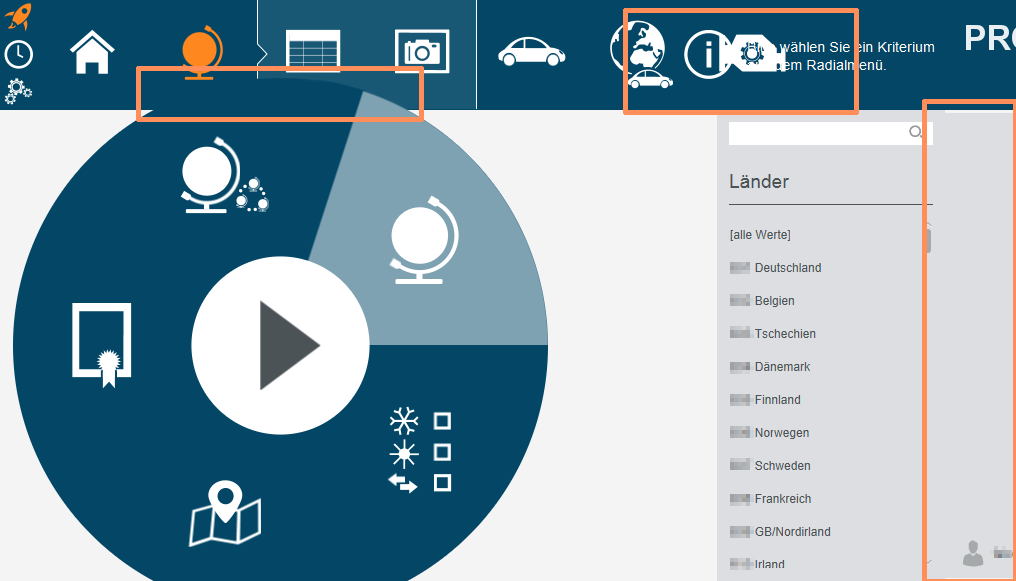
\includegraphics[width=0.6\textwidth]{grafiken/radial_bug.png}
 \caption{Layoutprobleme Hauptbildschirm}
 \label{fig:layoutMainScreen}
\end{figure}
Zur Behebung der allgemeinen Positionierungsprobleme im Hauptfenster muss das Layoutverhalten des Wurzelknotens verändert werden, sodass die Seitenleiste eine unveränderliche Position hat und diese nicht mehr durch die Position und Größe des Hauptinhaltes bestimmt wird. Die Komponenten dürfen keinesfalls außerhalb des sichtbaren Bereiches liegen. Innerhalb der Navigationsleiste kann das Problem so behoben werden, dass der Hilfetext anfänglich die Breite je nach verbleibendem Platz verringert und bei zu geringer Breite verschwindet. Bietet der Navigationsbereich wieder ausreichend Platz, erscheint der Hilfetext wieder. Als zweite Stufe wird selbiges Verfahren auf das Logo angewandt, dass bei zu geringer Größe ebenfalls Elemente verbirgt.\par
\heading{Filterbildschirm}
Auch hier stellten sich zwei verschiedene Probleme heraus. Das erste Problem ist die Position des Radialmenüs. Dieses überlagert, sobald der vorhandene Platz nicht mehr ausreicht, die Navigationsleiste. Zudem stellt sich in dem Filter für den LTÜ-Anwendungsfall der Umstand ein, dass zwei Schaltflächen zum Umschalten des Radialmenüs in der linken oberen Ecke des Radialmenüs vorhanden sind. Auch diese werden durch das Radialmenü verdeckt.\par
\begin{figure}[H]
 \centering
 
\includegraphics[width=0.4\textwidth]{grafiken/radial_bug2.png}
 \caption{Layoutprobleme LTÜ-Filter}
 \label{fig:layoutLtueFilter}
\end{figure}
Eine mögliche Lösung wäre, die Größe des Radialmenüs zu verringern, sobald der vorhandene Platz nicht mehr ausreicht. Dies widerspräche allerdings den Designrichtlinien, nach denen die Größe des runden Menüs exakt berechnet wurde, um im Einklang mit der Multi-Level-Liste und der Sidebar gesehen zu werden. Die andere Alternative ist es, das Verkleinern der Anwendung nur soweit zu erlauben, dass das Radialmenü noch in voller Größe (mit Abständen an allen Seiten) in dem Inhaltsbereich angezeigt werden kann. Dieser Wert liegt bei ungefähr 1024 x 768 Pixeln, was einer gängigen, jedoch geringen Monitor- oder Beamer-Auflösung entspricht.\par
Das Verkleinern der Auswahlbuttons ist ebenfalls keine Option. Durch das Begrenzen der Mindestgröße der Anwendung allerdings wird nur die rechte der beiden Schaltflächen verdeckt. Kollidieren durch das Verkleinern des Fensters das Radialmenü und besagte Schaltfläche, kann die Position des Buttons verändert werden. Er würde dann in der rechten oberen Ecke erneut auftauchen. Ist wieder ausreichend Platz vorhanden, kehrt die Schaltfläche an die ursprüngliche Position zurück. Unter normalen Umständen würde eine derartige Umsetzung nicht den Anforderungen genügen, da die Positionsänderung für leichte Verwirrung beim Anwender sorgen könnte, mangels Alternative muss die Umsetzung jedoch so erfolgen. Zudem ist sich der Nutzer bewusst, dass er bei starker Verkleinerung der Anwendung außerhalb der optimalen Benutzungsgröße arbeitet und nimmt das Risiko einer verringerten Usability im Austausch für die Individualisierbarkeit hin.\par
\heading{Ergebnisansichten}
Bei sämtlichen Ergebnisansichten fällt auf, dass diese sich bereits an die Größe des Inhaltsbereiches anpassen. In einigen Ansichten, wie der Ergebnistabelle und der Listenansicht wirken die Informationen bei kleineren Auflösungen jedoch stark gedrängt. Der Nutzer muss viel scrollen, um in dem kleinen Bereich die Werte angezeigt zu bekommen, nach denen er im Augenblick sucht. Um dies angenehmer zu gestalten, sollte es möglich sein, die Sidebar und die Navigationsleiste übergangsweise auszublenden und so die Ergebnisansicht auf dem gesamten verfügbaren Raum präsentiert zu bekommen. Das Verlassen dieser Präsentation kann durch einen hinzugefügten Button oder durch das Drücken der ESC-Taste erfolgen. Um zu dem Verständnis der Funktion beizutragen, erfolgt der Zustandswechsel animiert, indem die Navigationsleiste nach oben aus de Fenster fährt und die Sidebar nach rechts. Währenddessen \enquote{wächst} der Inhaltsbereich auf die gesamte Fenstergröße an.\par
\section{Umsetzung} \label{sec:responsiveImplementation}
Die Implementierung erfolgt auf Basis der Design-Entscheidungen des vorangegangenen Abschnittes.\par
\heading{Wurzel-Komponente}
Einige der Implementierungsaufgaben lassen sich zusammenfassen und durch die Implementierung einer neuen Komponente verwirklichen. Diese Komponente wird anstelle der derzeitigen Wurzel-Komponente der Anwendung eingesetzt. Zuvor bestand diese aus einer \textit{BorderPane}, die es erlaubt, Komponenten so anzuordnen, dass diese sich an den Seitenrändern orientieren und eine weitere \textit{Center}-Bereich ausfüllt. Eine ähnliche Komponente wird auch für das neue Verhalten benötigt.\par
Durch die Erweiterung der \textit{BorderPane}-Komponente würden so die Funktionalitäten dieser übernommen werden können und verändert, sowie weitere hinzugefügt werden können. So würden sich die meisten Layoutprobleme bei kleinen Fenstergrößen beheben lassen und zusätzlich die Vollbild-Funktion für die Ergebnisansichten eingebaut werden können.\par
Jeder JavaFX Container-Knoten implementiert eine Methode \textit{\#{}layoutChildren()}. Diese bestimmt jeweils, abhängig von einigen Eigenschaften, sowohl des Containers selbst, als auch des Inhaltes, die Position und Größe der beinhalteten Komponenten. Diese Methode kann überschrieben werden, um das Verhalten zu ändern. Die abgeleitete \textit{BorderPane}, die den neuen Wurzelknoten darstellt, überschreibt das Verhalten und berechnet die Position der Komponenten auf eine vergleichbare, aber dennoch eigene Weise. So wird erreicht, dass sich die Sidebar stets an dem äußeren rechten Rand befindet und nicht aus dem sichtbaren Bereich verschwindet, selbst, wenn die Mindestgröße der \textit{Center}- Komponente dadurch unterschritten wird. Durch das überschriebene Layoutverhalten wird der Position und korrekten Darstellung der Elemente eine höhere Gewichtung zuteil als der festgelegten Größe. Durch jene Veränderungen an der Größen- und Positionsberechnung wird ebenfalls verhindert, dass die Navigationsleiste überlagert wird.\par
Die Vollbildfunktion muss ebenfalls als Teil des Layoutverhaltens implementiert werden. Für die Positionsberechnung der Navigationsleiste und der Seitenleiste muss in Betracht gezogen werden, ob der Vollbildmodus aktiv oder inaktiv ist. Ist er inaktiv, kann die Positionsberechnung wie gewohnt ausgeführt werden. Bei aktivem Vollbildmodus muss die Position der Navigationsleiste und die Position der Sidebar im Nachhinein modifiziert werden, sodass die \textit{Center}-Komponente das gesamte Fenster zur Verfügung hat.\par
Damit der Übergang vom normalen Modus in den Vollbildmodus und zurück für den Nutzer plausibel ist, wird eine Animation verwendet. Diese sorgt dafür, dass sich die äußeren Elemente aus dem Fenster bewegen, während das mittlere Element wächst. Dies geschieht, indem ein Property (\textit{Vollbildfaktor}) durch eine JavaFX-Animation verändert wird. Es ändert den Wert beim Wechsel in dem Vollbildmodus von 0 zu 1 und von 1 zu 0, wenn der Modus wieder verlassen wird. Die JavaFX-Animation sorgt dafür, dass innerhalb einer gegebenen Zeitspanne (in diesem Fall 1 Sekunde) der Wert mehrfach verändert wird, bis der Zielwert erreicht ist. Ein \textit{Listener} auf dem \textit{Vollbildfaktor} sorgt dafür, dass bei jeder Aktualisierung des Wertes der Layout-Algorithmus erneut ausgeführt ist. Dieser zieht den Vollbildfaktor in Betracht und richtet die Elemente entsprechend aus.\par
Eine schematische Darstellung dieses Verfahrens ist in dem nachfolgenden Flussdiagramm festgehalten:
\begin{figure}[H]
 \centering
 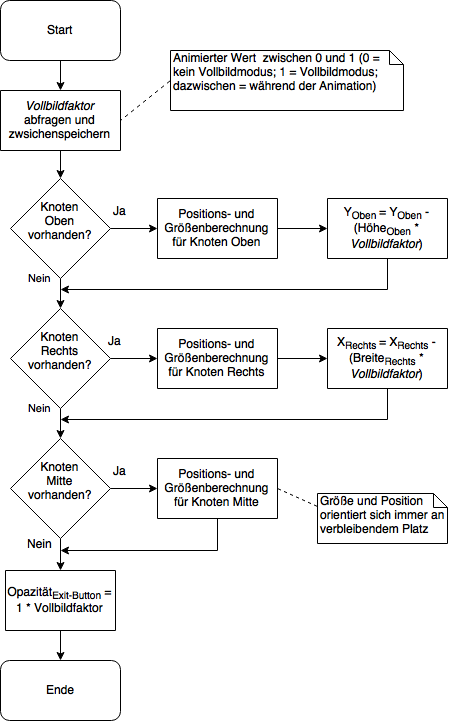
\includegraphics[width=0.75\textwidth]{grafiken/root_node_layout.png}
 \caption{Wurzelknoten Layoutverfahren}
 \label{fig:rootNodeLayout}
\end{figure}
\heading{Navigationsleiste}
Um in der Navigationsleiste die weniger wichtigen Elemente, sprich Infotext und Logo, sukzessive zu entfernen, wird ein Listener benötigt, der auf die Breiten-Property der gesamten Navigationsleiste lauscht. Verändert diese sich, wird eine Berechnung ausgeführt, die überprüft, ob noch genügend Platz für die einzelnen Elemente vorhanden ist. Ungeachtet der Implementierungsdetails, ist die Logik schnell erklärt:
\begin{itemize}
	\item Der Hilfetext wird angezeigt, wenn:
 		\begin{equation}
 			Breite_{Navi-leiste} >= Breite_{Navi-elemente} + Breite_{Logo} + MinBreite_{Hilfetext}
 		\end{equation}
 	\item Das Logo wird angezeigt, wenn:
 		\begin{equation}
	 		Breite_{Navi-leiste} >= Breite_{Navi-elemente} + Breite_{Logo}
 		\end{equation}
\end{itemize}
Damit das Logo bei Entfernen des Infotextes am rechten Rand der HBox, aus der die Navigationsleiste besteht, positioniert bleibt, wird ein unsichtbarer Platzhalter eingefügt, der stets die Breite des restlichen zur Verfügung stehenden Platzes einnimmt. Wird der Infotext wieder eingeblendet, wird der Platzhalter entfernt. Dies ist notwendig, da HBox-Container die Eigenschaft haben, alle beinhalteten Elemente horizontal direkt nebeneinander anzuordnen.\par
\begin{figure}[H]
 \centering
 
\includegraphics[width=0.8\textwidth]{grafiken/fix_nav.png}
 \caption{Schmale Navigationsleiste ohne Infotext}
 \label{fig:fixNav}
\end{figure}
\heading{LTÜ-Filter}
%\editHere{BLA}\par
Um den Button im LTÜ-Filterbildschirm repositionieren zu können, muss berechnet werden, ob das Radialmenü mit dem rechten der Auswahlbuttons kollidiert. Der Kollisionsalgorithmus nutzt die Radien der beiden betrachteten kreisförmigen Elemente (rechter Button und Radialmenü), um zu determinieren, ob die rechte der Schaltflächen die Position wechseln muss. Abhängig von der Breite und Höhe des Fensters wird dieser Wert aktualisiert. Ist eine Kollision vorhanden, muss der Button die Position ändern. Der Button erhält seine Ausgangsposition zurück, wenn die Berechnung von dem ursprünglichen Mittelpunkt und dem Radius der Schaltfläche eine Kollision ausschließt.\par
\begin{figure}[H]
 \centering
 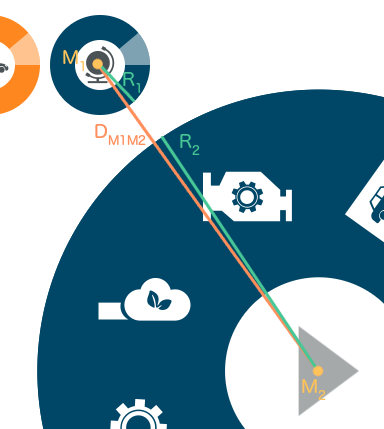
\includegraphics[width=0.4\textwidth]{grafiken/radius.png}
 \caption{Kollisionsberechnung im Filterbildschirm}
 \label{fig:collisionFilter}
\end{figure}
Eine Kollision liegt vor, wenn:\par
\begin{equation}
	D_{M1M2} <= R_1 + R_2 + Padding
\end{equation}
Das Padding bezeichnet den Mindestabstand zwischen den beiden Objekten. Liegt dieser bei 0, ist eine Kollision erst bei direktem Kontakt der Objekte gegeben.\par
Wird eine Kollision erkannt, wechselt der Button die Position auf die rechte Seite des Radialmenüs:
\begin{figure}[H]
 \centering
 
\includegraphics[width=0.5\textwidth]{grafiken/fix_filter.png}
 \caption{Alternative Buttonposition im LTÜ-Filter}
 \label{fig:fixFilter}
\end{figure}